The following sections are dedicated to the Camera Layer of this project. This layer includes Raspberry Pi Zero, database, stepper motor drivers, stepper motor, and camera module subsystems. The Camera Layer manages the actions set forth by the user in the Web Interface layer. The operating system used is Raspbian, while the programming language used is python. Besides the stepper motors components, a custom PCB board is used.

\subsection{Camera Layer}
The Raspberry Pi Zero will execute commands based on the user in the Web Interface layer. Once the user sets forth a command, the RPi Zero will execute and control the movements of the camera using the stepper motor driver to then control the stepper motors.

\subsection{Camera Layer Hardware}
Since the RPi zero has its own unique operating system, the operating system that will be used is Raspbian. 

\subsection{Camera Layer Software Dependencies}
Besides standard libraries that were installed, lwiringpi library had to be installed to allow functionality of the C++ code we were using at first to test the camera layer. Mjpeg will be used to as the video compressor since it would be the easier router for the amount of time to complete the project in the required time.The functionality is also dependent on the custom PCB stepper motor driver to control the stepper motors.


\subsection{Raspberry Pi Zero Subsystem}
The Raspberry Pi Zero is controlled by user input in the web interface layer, which is then responsible for controlling all other subsystems in the camera layer.


\begin{figure}[h!] 
 	\centering 
  	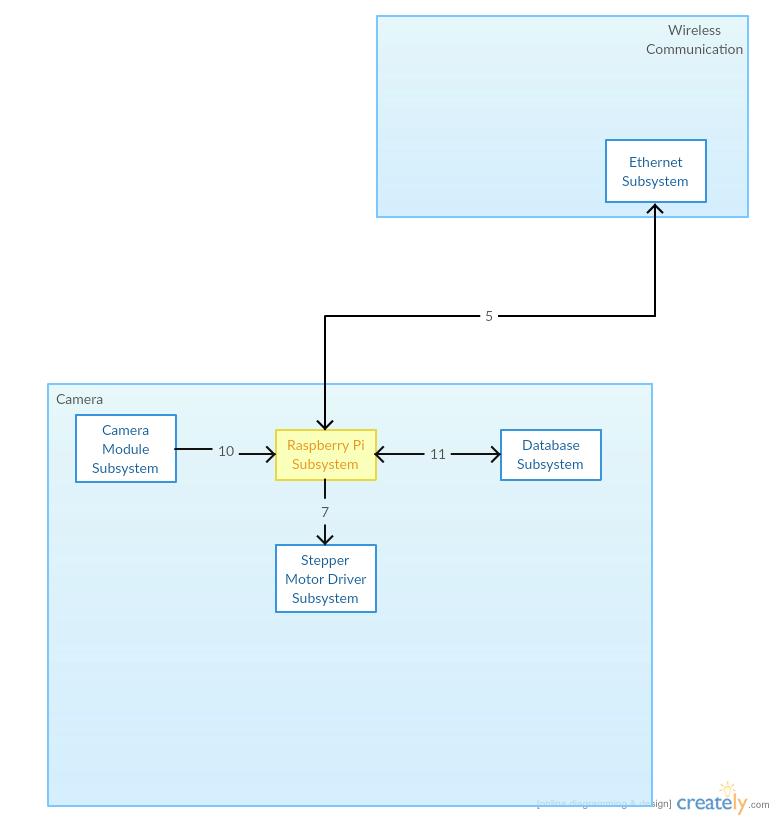
\includegraphics[width=0.60\textwidth]{architectural design specification latex/images/ADSdiagrams/raspberrypisubsystem.png} 
 \caption{Raspberry Pi Subsystem Description} 
\end{figure} 




\subsubsection{Raspberry Pi Subsystem Hardware}
The Rpi Zero has a 1Ghz single-core CPU, 512MB RAM, micro USB powered, and a 40 pin header HAT.

\subsubsection{Raspberry Pi Subsystem Operating System}
The required operating system is Raspbian.


\subsubsection{Raspberry Pi Subsystem Programming Languages}
The programming language used to control the Raspberry Pi Zero is Python and C++.

\subsubsection{Raspberry Pi Subsystem Data Structures}
For testing purposes and programming, the Raspberry Pi Zero is connected to a monitor via and HDMI and VGA connector.



\subsection{Database Subsystem}
The Rpi Zero has a wireless network card for internet connectivity, so all the information sent and received by the Raspberry Pi Zero is stored in the database, which is used to store logs of important information.

\begin{figure}[h!] 
 	\centering 
  	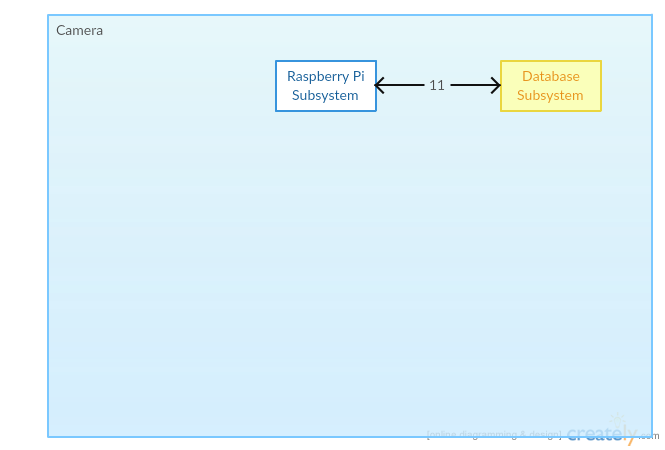
\includegraphics[width=0.60\textwidth]{architectural design specification latex/images/ADSdiagrams/databasesubsystem.png} 
 \caption{Database Subsystem Description} 
\end{figure}


\subsection{Stepper Motor Driver Subsystem}
The stepper motor driver is essentially software installed on the Raspberry Pi Zero to control the stepper motors and allow the stepper motors to work.

\begin{figure}[h!] 
 	\centering 
  	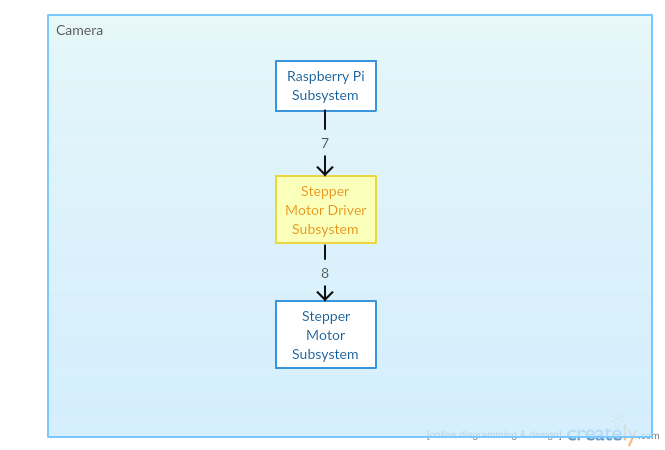
\includegraphics[width=0.60\textwidth]{architectural design specification latex/images/ADSdiagrams/steppermotordriversubsystem.png} 
 \caption{Stepper Motor Driver Subsystem Description} 
\end{figure}


\subsubsection{Stepper Motor Driver Subsystem Software Dependencies}
The stepper motor driver is dependent on the Raspberry Pi Zero programmed by the developer.

\subsubsection{Stepper Motor Driver Subsystem Programming Languages}
The stepper motor driver uses Python programming language to control the stepper motors.



\subsection{Stepper Motor Subsystem}
The stepper motor driver is essentially software installed on the RPi Zero to control the stepper motors. The stepper motors are connected to the GPIO in the RPi Zero through wires. The stepper motors are controlled through the user web interface. The stepper motors can pan and tilt the camera module. 

\begin{figure}[h!] 
 	\centering 
  	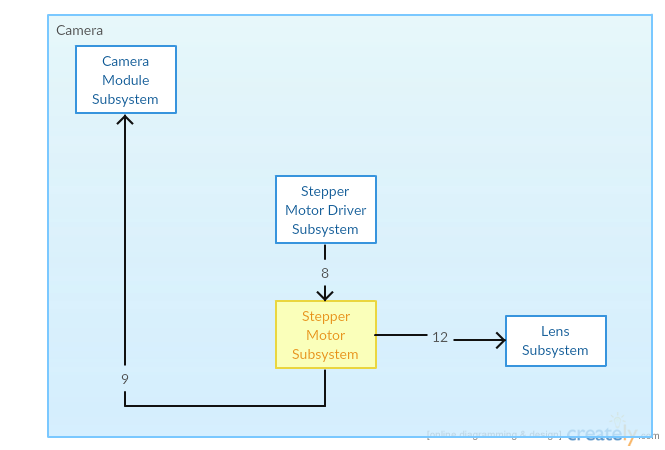
\includegraphics[width=0.60\textwidth]{architectural design specification latex/images/ADSdiagrams/steppermotorsubsystem.png} 
 \caption{Stepper Motor Subsystem Description} 
\end{figure}

\subsubsection{Stepper Motor Subsystem Hardware}
The team created a custom PCB board HAT which allows more room to house the stepper motors inside the camera dome. The HAT mounts on top of the RPi Zero and then female to female wires running from the HAT to the stepper motors allows the connection between the two.


\subsubsection{Stepper Motor Subsystem Software Dependencies}
The stepper motors are dependent on the stepper motor driver and the way the developer programmed the functionality of the stepper motors.


\subsubsection{Stepper Motor Subsystem Data Structures}
A stepper motor is a brushless, synchronous electric motor that converts digital pulses into mechanical shaft rotations. Each rotation of a stepper motor is divided into a set number of steps.



\subsection{Camera Module Subsystem}
The camera module is controlled by the stepper motor, which moves the camera (pan and tilt) certain degrees based on user interactions.The camera module is responsible for capturing images of the surrounding landscape. The camera module will provide live feedback of its surroundings when the user request the information from the web interface.

\begin{figure}[h!] 
 	\centering 
  	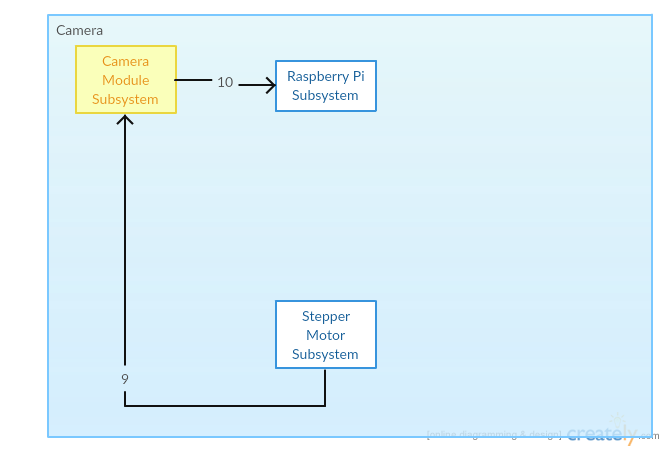
\includegraphics[width=0.60\textwidth]{architectural design specification latex/images/ADSdiagrams/cameramodulesubsystem.png} 
 \caption{Camera Module Subsystem Description} 
\end{figure}

\subsubsection{Camera Module Subsystem Hardware}
The camera module is a special connection that can only be made to the RPi Zero.


\subsubsection{Camera Module Subsystem Software Dependencies}
Since the camera module can only be used by the RPi zero, the camera module depends on the pre-installed software of the RPi zero.


\subsubsection{Camera Module Subsystem Data Structures}
The camera module has a five megapixel fixed-focus camera that supports 1080p, 720p and VGA90 video modes, as well as stills capture. It attaches via a 15cm ribbon cable to the CSI port on the RPi Zero.
